\section{Implementation}
\label{sec:implementation}

To test whether it is possible to prioritize PRs we have designed a service that automatically tries to do just that.

\subsection{Architecture}

Our implementation of the service consists of several components.
Figure \ref{fig:architecture} shows a global overview of the architecture.
The \prioritizer service uses two main data sources: GitHub and the \ghtorrent project.
The latter provides a message queue which can be used to subscribe to pull request events.
When such an event arrives the \emph{watcher} component of the \prioritizer is notified (1) and starts prioritizing the project (2).
When the \emph{analyzer} gets a prioritization request it fetches an up-to-date list of PRs from GitHub (3).
At the same time it fetches the pull request contents to the local Git repository.
When the data is fetched the analyzer starts enriching the PR list with data from the local repository and \ghtorrent (4).
This step calculates and adds several of the features to the PRs.
The data is now ready to be processed by the \emph{predictor} (5) which gives a certain rank to the PRs.
After the ordered list is returned to the analyzer (6), the output is generated and available for the \emph{visualizer} (7).

\begin{figure}
  \centering
  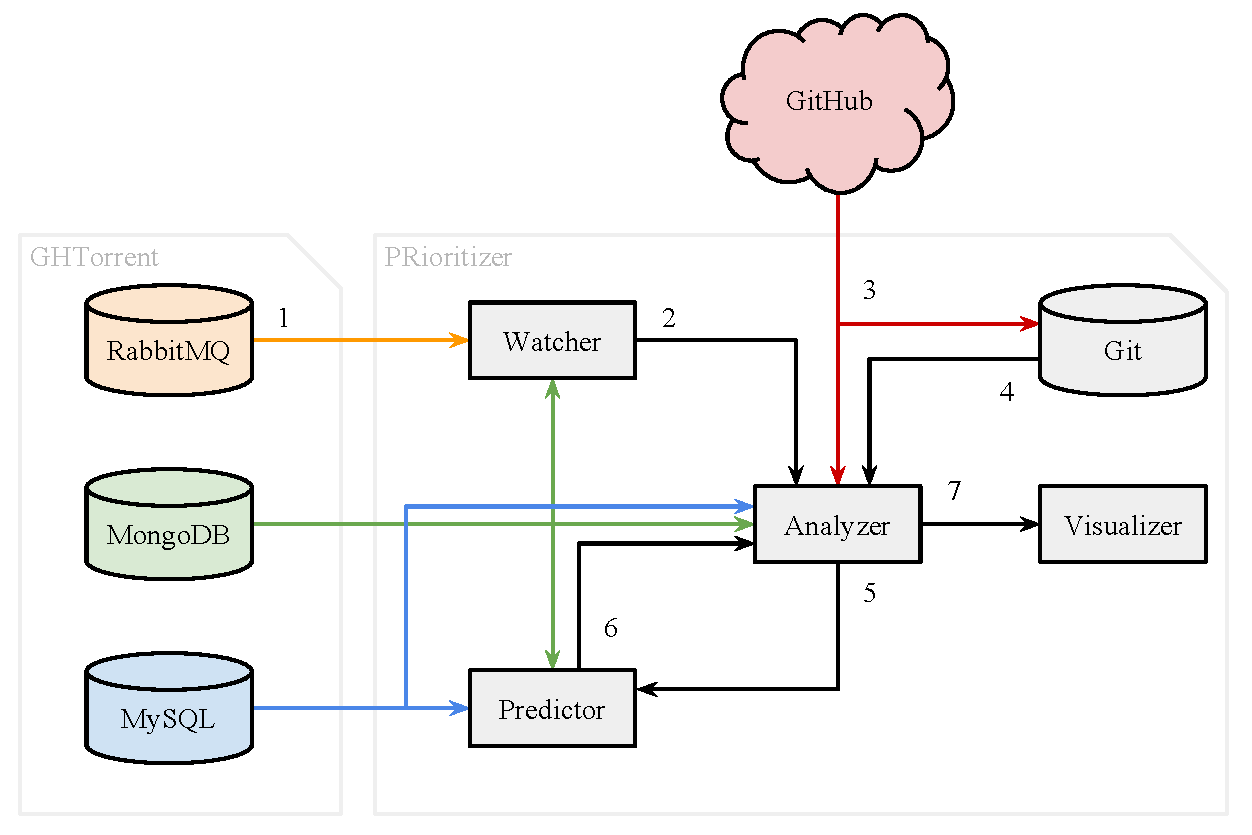
\includegraphics[width=0.5\textwidth]{../figs/architecture.pdf}
  \caption[Diagram of the architecture]
   {Diagram of the architecture. It shows the different data sources and components used by the \prioritizer service.}
  \label{fig:architecture}
\end{figure}

